% File project.tex
%% Style files for ACL 2021
\documentclass[11pt,a4paper]{article}
\usepackage[hyperref]{acl2021}
\usepackage{times}
\usepackage{booktabs}
\usepackage{todonotes}
\usepackage{latexsym}
\renewcommand{\UrlFont}{\ttfamily\small}
\usepackage{multirow}

% This is not strictly necessary, and may be commented out,
% but it will improve the layout of the manuscript,
% and will typically save some space.
\usepackage{microtype}

\aclfinalcopy 

\newcommand\BibTeX{B\textsc{ib}\TeX}

\title{11-777 Spring 2021 Class Project\\
Action Feasibility in the ALFRED Task}

\author{
  Christian Deverall\thanks{\hspace{4pt}Everyone Contributed Equally -- Alphabetical order} \hspace{2em} Jingyuan Li $^*$ \hspace{2em} Artidoro Pagnoni $^*$ \\
  \texttt{\{cdeveral, jingyua4, apagnoni\}@andrew.cmu.edu}
  }

\date{}

\begin{document}
\maketitle

\begin{abstract}
    The task of navigating a room to complete household tasks defined with natural language remains challenging for AI systems. In this project, we focus on the ALFRED dataset. We perform an in-depth analysis of the dataset, evaluate two competitive models, and identify their limitations. We find that even the best of these two models, MOCA, outputs a significant number of infeasible actions. We evaluate whether providing MOCA with a better action feasibility module improves the overall performance by reducing the infeasible actions taken by the agent.
\end{abstract}

\section{Introduction}
Understanding and following task-oriented instructions are natural and straightforward skills for human beings. This remains to a great challenge for robotic systems due to the difficulties in both visual and linguistic understanding. In this project we focus on the ALFRED dataset \cite{ALFRED20} to explore the navigation and interaction of robot agents. The high-level task for the ALFRED dataset is to predict the correct sequence of household actions given textual instructions and visual feedback. It is unique in that the actions are long, compositional, and non-reversible. An example of this is that the agent must pick up a knife to slice a potato. Moreover, once a potato is sliced, it cannot be put back together. Actions consist of navigation within a room or interaction with an object. For interaction, a pixel-wise mask must be predicted whereby the object with the highest intersection-over-union score with the interaction mask is acted upon. The textual instructions come in the form of both high-level task descriptions and step-by-step commands. The visual feedback is ego-centric and the next image is provided after each action is performed. Compared to previous datasets, the ALFRED dataset contains a diverse range of tasks. Specifically, there are 7 high-level task types parameterized by a combination of 84 object classes and 120 household scenes.

In the ALFRED world, actions are not always valid. This may be due to a variety of reasons, for example, objects could be blocking the movement of the agent, or an object the agent may want to interact with  may not be present in the image.  While it is natural for humans to avoid taking such mistaken actions, it is challenging for the trained AI agents since they are not aware of the consequence of an action. An intuitive explanation for such inability is that the training paths don't involve any examples of actions that are not feasible. The agent is only provided with indirect information about action feasibility: it is guaranteed that all actions in the training trajectories are feasible and has to deduce by lack of examples including some actions that are not feasible. As a result, the agent tends to make mistakes when it's under new environments since they have no knowledge that tells them making mistakes leads to failure. As a reference, we observed that 28\% and 40\% (for seen and unseen scenes respectively) of trajectories are interrupted in MOCA \cite{singh2020moca} because they reach the limit of 10 errors. This indicates that the presence of many invalid actions causes a large portion of failures.

To help the agent make better decisions on action selection, we identify modeling action feasibility as an interesting avenue for improvement. This direction is particularly challenging in the context of Seq2Seq models such as those that have been employed in the ALFRED task since it requires the agent to not only understand correct paths but also understand incorrect actions. To achieve this goal, we propose to build methods that inform the feasibility of an action. Building such a model requires extra data that comprehensively describes the action spaces to an extent that is greater than what is given in the original Alfred dataset. To reach this goal, we collect a large set of image-action pairs that describe the action feasibility in each location in a room. With the data, we then trained a module to predict the feasibility of action. While simple, we verify that this model is effective in predicting the action feasibility in both seen and unseen spaces, demonstrating the feasibility of our hypothesis. Besides, we also tested the potential by informing the agent about action feasibility, where a clear improvement is demonstrated in tasks performed in unseen spaces.


% \begin{table*}[]
% \centering

% \begin{tabular}{|l|c|c|c|c|}
% \hline
%                                              & \multicolumn{2}{c|}{Seen} & \multicolumn{2}{c|}{Unseen} \\ \hline
%                                              & Failure     & Success     & Failure      & Success      \\ \hline
% Agent blocked                                & 1514        & 139         & 2639         & 7            \\ \hline
% Agent state not allowed                      & 127         & 2           & 79           & 0            \\ \hline
% Object visible but not located correctly     & 1569        & 28          & 2191         & 3            \\ \hline
% Object not found in scene                    & 96          & 0           & 202          & 4            \\ \hline
% Object property not allowed                  & 170         & 9           & 102          & 2            \\ \hline
% Others                                       & 163         & 0           & 124          & 0            \\ \hline
% Target state not allowed                     & 105         & 0           & 46           & 0            \\ \hline
% No valid target                              & 40          & 0           & 25           & 0            \\ \hline
% Object not visible                           & 109         & 3           & 153          & 0            \\ \hline
% Object state not allowed                     & 21          & 0           & 18           & 2            \\ \hline
%                                              &             &             &              &              \\ \hline
% Frequency of error limit (10 errors) reached & 0.28        &             & 0.40         &              \\ \hline
% Number of Errors (when less then 10 errors)  & 4.44        &             & 4.91         &              \\ \hline
% Average number of errors                     & 6.03        & 1.05        & 6.99         & 0.78         \\ \hline
% Average length of sequences of errors        & 2.954       & 1.19        & 3.57         & 1.17         \\ \hline
% \end{tabular}
% \caption{Analysis of types of error messages returned by Thor for invalid actions. We compare failed and successful tasks as well as unseen and seen scenes. The first part of the table contains counts of errors of different types across the validation dataset. The second part computes statistics about the number of errors per trajectory.}
% \label{tab:error_analysis}
% \end{table*}

\section{Task Background}
In this section, we present an analysis into the dataset and two baseline models. Our objective is to get a sense of the types of demonstrations that are present in the ALFRED dataset as well as examine the weaknesses and strengths of the current state-of-the-art models.

\subsection{High-level Analysis}

\paragraph{Action-Space} In the ALFRED dataset, tasks are described by low-level and high-level actions. In this section, we examine the patterns behind these actions and the objects which are acted upon. In order to gauge the size of tasks and the granularity of actions, we provide statistics about the number of low-level and high-level actions per task in \autoref{tab:number_actions}.


\begin{table}[]
    \centering
    \resizebox{\linewidth}{!}{
\begin{tabular}{lrrrr}
\toprule
     split &  mean &  std &  min &  max \\
\midrule
    low-level train &  49.78 & 24.78 &    5 &   234 \\
    low-level val seen &  46.98 & 20.22 &    13 &   137 \\
    low-level val unseen & 50.12 & 25.61 &    12 &   165\\
    high-level train &  6.51 & 2.49 &  2 &   19 \\
    high-level val seen &  6.47 & 2.62 &    3 &   16 \\
    high-level val unseen &  6.16 & 2.33 &    3 &   14 \\
\bottomrule
\end{tabular}
}
    \caption{Statistics on the number of low-level and high-level actions for the splits of the data.}
    \label{tab:number_actions}
\end{table}

Low-level actions are often repeated in order to fully complete a high-level goal. For example, numerous fixed-distance movement actions are required to travel from one end of the kitchen to the other. This repetition pattern is relevant to action prediction because for highly repeated actions, it is likely that the next action is the exact same as the current one. In \autoref{fig:duplicate_dist}, it can be seen that by far the most duplicated action is the "MoveAhead" operation encompassing approximately 44\% of all actions.

\begin{figure}
    \centering
    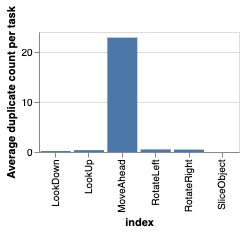
\includegraphics[width=\linewidth]{Reports/1-Task-Definition-and-Data/duplicate_distrib.png}
    \caption{Average number of duplicate actions per task}
    \label{fig:duplicate_dist}
\end{figure}


\paragraph{Instruction-based Analysis}
There are two types of instructions: the task description and the detailed instructions. The task description is generally a single sentence outlining the goal of the task while the detailed instructions break the task down into sub-goals and provide a sentence instruction for each sub-goal. We measure statistics on the number of sub-goals for each task in \autoref{tab:sub_goals}. We observe that there are up to 19 distinct sub-goals in each trajectory and that on average there are 6.7 sub-goals. The tasks are not simple as they require a minimum of three sub-goals.

\begin{table}[]
    \centering
\begin{tabular}{lrrrr}
\toprule
     split &  mean &  std &  min &  max \\
\midrule
     train &  6.72 & 2.49 &    3 &   19 \\
  val seen &  6.79 & 2.73 &    4 &   16 \\
val unseen &  6.26 & 2.33 &    4 &   14 \\
\bottomrule
\end{tabular}
    \caption{Statistics on the number of sentence instructions (sub-goals) for the splits of the data.}
    \label{tab:sub_goals}
\end{table}



\subsection{Analysis of Baselines}

The baselines we evaluate are the ``Modular Object-Centric Approach'' (MOCA) \citep{singh2020moca} model and the ``Sequence-to-Sequence with Progress Monitor'' model (baseline of the ALFRED proposal paper) \citep{ALFRED20}. We provide comparisons in two settings: ``seen'' and ``unseen''. ``Seen'' refers to when all the test tasks take place in rooms that have been previously seen in the training set.

\paragraph{Feasible Action Analysis} In the ALFRED world, actions are not always feasible. This might be due to a variety of reasons, for example, objects could be blocking the movement of the agent, or an object the agent wants to interact with might not be present in the image.   
In Table \ref{tab:error_analysis}, we report statistics on the reason why certain actions are considered invalid for the MOCA model. Our first observation is that in the seen scenes  the vast majority (80\%) of invalid actions are from two categories: the agent is unable to move (blocked) and the object was visible but not located correctly. In the unseen scenes this trend in the errors is even more accentuated with   87\% of the errors being from these two categories  (47\% for the agent being blocked, and 40\% for the object not being located correctly). These results indicate possible areas for improvement.

Furthermore, in the second part of the Table \ref{tab:error_analysis}, we observe that 28\% and 40\% (for seen and unseen scenes respectively) of trajectories are interrupted because they reach the limit of 10 errors. This indicates that the presence of many invalid actions causes a large portion of failures. The two major areas for improvement in this direction are: 1. spatial detection of the validity of an action and 2. visual detection of objects. The fact that the trajectories predicted by the MOCA model contain so many infeasible actions provides the central motivation for our research, to provide the model with an awareness of whether predicted actions are feasible or infeasible.

\begin{table*}[]
\centering

\begin{tabular}{|l|c|c|c|c|}
\hline
                                             & \multicolumn{2}{c|}{Seen} & \multicolumn{2}{c|}{Unseen} \\ \hline
                                             & Failure     & Success     & Failure      & Success      \\ \hline
Agent blocked                                & 1514        & 139         & 2639         & 7            \\ \hline
Agent state not allowed                      & 127         & 2           & 79           & 0            \\ \hline
Object visible but not located correctly     & 1569        & 28          & 2191         & 3            \\ \hline
Object not found in scene                    & 96          & 0           & 202          & 4            \\ \hline
Object property not allowed                  & 170         & 9           & 102          & 2            \\ \hline
Others                                       & 163         & 0           & 124          & 0            \\ \hline
Target state not allowed                     & 105         & 0           & 46           & 0            \\ \hline
No valid target                              & 40          & 0           & 25           & 0            \\ \hline
Object not visible                           & 109         & 3           & 153          & 0            \\ \hline
Object state not allowed                     & 21          & 0           & 18           & 2            \\ \hline
                                             &             &             &              &              \\ \hline
Frequency of error limit (10 errors) reached & 0.28        &             & 0.40         &              \\ \hline
Number of Errors (when less then 10 errors)  & 4.44        &             & 4.91         &              \\ \hline
Average number of errors                     & 6.03        & 1.05        & 6.99         & 0.78         \\ \hline
Average length of sequences of errors        & 2.954       & 1.19        & 3.57         & 1.17         \\ \hline
\end{tabular}
\caption{Analysis of types of error messages returned by Thor for invalid actions. We compare failed and successful tasks as well as unseen and seen scenes. The first part of the table contains counts of errors of different types across the validation dataset. The second part computes statistics about the number of errors per trajectory.}
\label{tab:error_analysis}
\end{table*}
% continue here

%\section{Conclusion}
%In this report, we analyze the ALFRED \cite{ALFRED20} dataset. We explore both the actions and the instructions in the training and validation data splits.
%We observed a highly imbalanced distribution of actions, and of action pairs, which indicates potential biases in the dataset. Strong symmetry is observed in the interactive actions that change the states of object, meaning potential rule-of-thumb that could be exploited in designing our own method.
%With respect to the instructions, we observe that almost all objects and verbs are common to the training and validation data splits. Furthermore, we see that there are long tailed distributions of nouns and verbs. Finally, the high-level task description includes more mentions of objects to specify the actions beyond the objects acted on.


\section{Related Work}
In this section, we investigate existing work related to our project. We focus on related techniques and tasks. The supporting techniques discussed here are (1) program synthesis/induction, (2) language-image grounding. The related task discussed here is multimodal embodied interaction.

\subsection{Program Synthesis}
One challenge of dealing with instructions expressed in natural language is that natural language is noisy. The same instructions can be expressed through different paraphrases and depending on the context the same instructions might describe different actions. The task of parsing natural language instructions into a representation that has a deterministic execution is generally referred to as program synthesis or inductive programming \citep{summers1977methodology, muggleton1994inductive}. 

\paragraph{Neural Code Generation} Previous work in program synthesis has explored the task of parsing natural language descriptions into source code written in a general-purpose programming language. \citet{yin2017syntactic} proposes a neural architecture which uses a grammar to explicitly capture the syntax of the target language in an Abstract Syntax Tree. \citet{dong2018coarse} use a different approach which is based on coarse-to-fine decoding and decomposes the parsing process into two stages: a rough sketch of the meaning of input utterance is first generated, and it is further refined by filling in the missing information at a second stage.

\paragraph{Compositionality} Instructions and questions are generally compositional. Being able to capture the compositional linguistic structure of natural language questions can help create and combine specialized modules. 
\citet{andreas2016neural} uses a natural language parser to dynamically lay out a network composed of reusable modules that are jointly trained. The CLEVR dataset \citep{johnson2017clevr} was proposed to test model's ability to perform compositional reasoning such as recognizing novel attribute combinations. In this sense it is similar to the ALFRED \citet{ALFRED20} instructions which test the performance of an agent in new action-object-scene combinations. \citet{santoro2017simple} propose Relation Networks to augment CNNs and perform relational reasoning on the CLEVR dataset.


\paragraph{Semantic Parsing} The problem of code program synthesis is related to semantic parsing where a natural language sentence is mapped into a cpmplete, formal meaning representation \citep{mooney2007learning}. Several approaches have been proposed to leverage unlabeled data for the task of semantic parsing using question-answering and paraphrase models
\citep{berant2013semantic, berant2014semantic} .

\subsection{Image Understanding}

\paragraph{Natural Language Object Retrieval}
Traditional image recognition tasks such as object detection and semantic segmentation have performed extremely well when the textual input is highly defined. Often bounding boxes and segmentation masks are directly associated with a tag or label that defines the object. One limitation of this method is that it cannot not leverage the complex structural information inherent to natural language. In \cite{vis_grounding}, natural language object retrieval is performed on a relatively small dataset using weak supervision. More specifically, the authors represent sentences as a parse tree, which enables learning at several levels of the tree for the same image caption. This method outperformed baselines that did not consider linguistic structure on the MS COCO and Visual Genome datasets. For the same task, \citep{end_to_end_approach} uses deep reinforcement learning to iteratively reshape a bounding box to localize the object. 

\paragraph{Visual QA} In contrast to the previous papers which only localize objects within images, the visual question answering task involves answering a more complex question about the image. In \citep{VQA}, which initially proposed the VQA task, the best performing model uses an LSTM to separately encode the text while a CNN encodes the image. \citep{stacked_attention} improves on this by introducing stacked attention networks, which iteratively queries the image. By repeatedly refining queries that combine both image and textual data, the latter attention layers can focus on the most relevant parts of the image. Recently, papers such as \cite{Wu_Liu_Wang_Li_2019} have provided innovations in the way that the image and textual encodings are fused together. Typical models take the product between both encodings, however this paper proposes the idea that the product of the difference between feature elements is a superior fusion.

\subsection{Multimodal Embodied Interaction}
The ability to understand and follow instructions is of great importance for robotic systems that aims to assist human in the real world. For its practicability, methods allowing the robots to follow instructions and complete specific goals have attracted great attention. One of the related tasks is called visual language navigation, which aims to generate sequences of actions from human instructions that guide the agent to complete tasks in specific scenes. The Room-to-Room dataset was proposed to simulate the real-world circumstance where instructions, scene images, and corresponding actions are provided, to accelerate the development of visual language navigation \cite{anderson2018_a}. To deal with the visual language navigation task, the multi-modal mapping between action sequence and instructions is built, which not only allows the agent to plan before taking actions but also enables data augmentation which improves the robustness of the model \cite{fried2018_a}. To allow the learning from environmental exploration and failure experiences, reinforcement learning techniques are also used in the navigation task \cite{ma2019_a, wang2018_a}. Besides performance improvements, many related works are also working on addressing specific assumptions made in the Room-to-Room dataset, including the discrete space assumption \cite{krantz2020_a}, and the known environment assumption \cite{tan2019_a}. While the Room-to-Room dataset has modeled VLN tasks comprehensively, one limitation that cannot be addressed is the lack of interaction which is one of the eventual goals of real-world robotic systems. To take a step forward, the ALFRED dataset is proposed \cite{shridhar_a}, with both navigation and interaction taken into consideration. Due to the requirement of interaction, the agent needs not only to decide the actions to take but also to figure out which object in the environment should be acted on, introducing extra complexity to the already hard problem. To address the issue, MOCA \cite{singh2020moca} with modules dealing with visual perception and action policy was proposed, to make the task feasible by dividing different components of the targets. The above describes works and tasks related to our project. In this project, we are intended to work on the exploration of and interaction with environment by the agent.



%\section{Motivation and Challenges}
%In the ALFRED world, actions are not always valid. This might be due to a variety of reasons, for example, objects could be blocking the movement of the agent, or an object the agent wants to interact with might not be present in the image.   
%In the previous report, we computed statistics on the cause for an action to be invalid for the MOCA model (statistics reported in Table \ref{tab:error_analysis}).
%Our main observation was that in both seen and unseen scenes that majority of invalid actions are due to two categories: the agent is unable to move (blocked) and the object is visible but not located correctly by the interaction mask. 

%We also observed that 28\% and 40\% (for seen and unseen scenes respectively) of trajectories are interrupted because they reach the limit of 10 errors. This indicates that the presence of many invalid actions causes a large portion of failures. The two major areas for improvement in this direction are: 1. spatial detection of the validity of an action and 2. visual detection of objects for improved interaction validity.

%Based on these observations, we identify modeling action feasibility as an interesting avenue for performance improvement. This direction is particularly challenging in the context of Seq2Seq models such as those that have been employed in the ALFRED task. It is not trivial to train a Seq2Seq model that follows a golden trajectory and expect it to learn about the feasibility of actions in the ALFRED environments. The training paths don't involve any examples of actions that are not feasible. The agent is only provided with indirect information about action feasibility: it is guaranteed that all actions in the training trajectories are feasible and has to deduce by lack of examples including some actions that they are not feasible. Solving this challenge will be the primary focus of our work.

%One overly naive approach to solve the problem is to simply decouple the action feasibility model and the action prediction model. Intuitively, a unimodal model that only uses visual cues could determine the feasibility of certain actions in a given space. This unimodal model could be used in combination with the action prediction component and ensure the most likely action that is feasible is chosen. However, this approach does not help the model obtain a better grounding of language and vision and become better at navigating its world. In our proposed approach, we do recommend using such module at inference time to avoid performing infeasible actions but we will focus on improving the Seq2Seq action prediction model itself.

%Furthermore, we find that improving the modeling of action feasibility is most interesting in the multimodal context of the ALFRED task. In particular, by better understanding the feasibility of actions in relation to both language and vision cues, we believe that the agent might be able to better generalize its understanding to unseen environments especially. For example, in the instruction ``walk along the kitchen counter'', the agent might understand that the use of ``walking along'' generally indicates that there is an object that cannot be traversed next to it which in this case is the ``kitchen counter''. On one hand this allows the agent to better understand the semantic of the instructions, but also hopefully allows the agent to generalize its understanding of action feasibility to unknown objects. If in an unseen environment an instruction requires the agent to ``walk along the sofa'', by association to the training example of the kitchen counter, the agent would learn about the feasibility of walking into the sofa.

%In summary, we believe that modeling action feasibility could both help improve performance by, among other things, providing a better grounding of the language instructions in the context of the multimodal ALFRED task.

\section{Proposed Approach}

After performing an analysis of the two baselines ``Modular Object-Centric Approach'' (MOCA) \citep{singh2020moca} model and  ``Sequence-to-Sequence with Progress Monitor'' model (baseline of the ALFRED proposal paper) \citep{ALFRED20}, we identify some areas that could lead to performance improvements. In this report we explain in detail what specific limitations were of greatest interest to our team in the context of a multimodal machine learning class, and how we plan to mitigate these limitations for the MOCA model.  

The proposed approach involves improving the model's understanding of its surrounding, in particular, its understanding of the feasibility of actions. We also propose two other approaches which are meant to improve the quality of the predicted mask which was one of the sources of action infeasibility.

\subsection{Action Feasibility Auxiliary Prediction}
Along with predicting the next action in MOCA, we propose an auxiliary prediction task. The model predicts which actions are feasible at each time step along the golden trajectories provided in the training set. 
We gather the data on which actions are feasible at each time step of the golden trajectories by querying the simulator offline before training. 
The current prediction task only requires the agent to predict the next best action to undertake and does not provide any clue to the model about any other differences in the available actions. Our hypothesis is that with the auxiliary action feasibility prediction task, the agent would develop an understanding of the available actions beyond whether they are the best next step but whether they are also feasible.

To achieve this goal, we define an auxiliary loss function that tells the agent about feasible and infeasible actions. In specific, in the Action Policy Module of MOCA, we add an extra linear layer before the action output, denoted as $\hat{A}$, representing the feasibility of the action. We want the agent to learn from the environment which action is feasible at each time step. And each element in $\hat{A}$ is activated by sigmoid function $\sigma$. We train this additional layer using focal loss \cite{lin2017focal}:

\begin{equation}
\begin{split}
    & Loss = -\frac{1}{n_a} \sum_{i=1}^{n_a} a^{i} (1 - \hat{a}^{i})^{\gamma} log (\hat{a}^{i}) \\
    & + (1 - a^{i}) \hat{a}^{i}^{\gamma} log (1 - \hat{a}^{i})
\end{split}
\end{equation}

where $\gamma$ is a tunable parameter. Here we use focal loss instead of conventional binary cross entropy loss because most actions are feasible and only a minority of actions are not feasible. Focal loss helps to reduce the influence of imbalanced samples.

% Why this is multimodal: Intuitively, the loss function above not only stresses the infeasibility of actions but also stresses the optimal actions. The optimal actions are informed by both the high-level instruction (eventual goal), and the low-level instruction (short-term goal), which is thus influenced by multi-modal data. Hopefully, the model will learn a better alignment between language, image, and its understanding of what can be done in the world.


\subsection{Action Feasibility Mask}
We propose a second stand-alone model that only uses the visual input and the interaction mask to predict the feasibility of an action. This model can be trained in a supervised fashion using the simulator sampling different locations and querying the feasibility of actions at those locations. 

Since the second model requires only visual input and action feasibility output independent of the previous step, the model can be trained offline. To train this model, we need a group of images ${I_1, I_2, ..., I_t}$ pre-collected from the simulator, and the corresponding action feasibility labels ${F_1, F_2, ..., F_t}$ at the location where the corresponding images are collected. The action feasibility in $F_n$ is 1 if the action is either a feasible navigational action or a feasible interactive action that acts on any objects in $I_n$, otherwise, it's 0. Given a visual feature extractor (e.g. ResNet, DenseNet) $\Phi(\o=cdot)$, we assume the output in the last layer of the model to be $F_{logits}$ of size $n_a$, where $n_a$ is the number of action. $F_{logits}$ is the score of action feasibility without any activation functions (i.e. it's the output from a linear layer). Then we generate the eventual action feasibility mask using the element-wise sigmoid function $\sigma$, i.e.

\begin{equation}
    \hat{F} = \sigma(F_{logits})
\end{equation}

Then we use the binary cross-entropy loss on each action for calculating the loss function, i.e. 

\begin{equation}
    Loss = -\frac{1}{n_a} \sum^{n_a}_{i=0} F^i log (\hat{F}^i) + (1-F^i) log ((1-\hat{F}^i))
\end{equation}
where $F^i$ is the feasibility of the $i^{th}$ action. By optimizing this target, we are able to train a module to tell the action feasibility.

After the module is trained, we are able to use it for better inference. In specific, given the action preference prediction given by the module to be $\hat{A}$, the initial strategy to select action is 

\begin{equation}
    a* = \argmax(\hat{A})  
\end{equation}

To avoid bad actions, we now select the target action through

\begin{equation}
    a* = \argmax(\hat{A}\odot\hat{F})
\end{equation}
where $\odot$ is element-wise multiplication.

% \subsection{Improved Instruction Use}

% The model architecture for the MOCA paper is provided in figure \ref{fig:sys_arch}. As can be observed, the Visual Perception Module does not receive input from the step-by-step instructions. Its input consists solely of the high-level goal statement, the image embedding and the previously predicted action. This omission could explain our finding that one of the most common sources of invalid actions is when ``the object is visible but not located correctly by the interaction mask''. As a result, the equation for $h_{t,m}$ would change to the following:

% \begin{equation}

%     h_{t,m} = LSTM_{m}([\hat{v}_{t,goal};\hat{x}_{t,goal};a_{t-1};\hat{x}_{t,instr}])

% \end{equation}

% where (similarly to the notation of the MOCA paper) [;] represents concatenation, $\hat{v}_{t,goal}$ represents the attended visual features, $\hat{x}_{t,goal}$ represents the attended features for the high-level goal, $;a_{t-1}$ represents the previously predicted action and $\hat{x}_{t,instr}$ represents the attended features for the step-by-step instruction. 

% \begin{figure*}
%     \centering
%     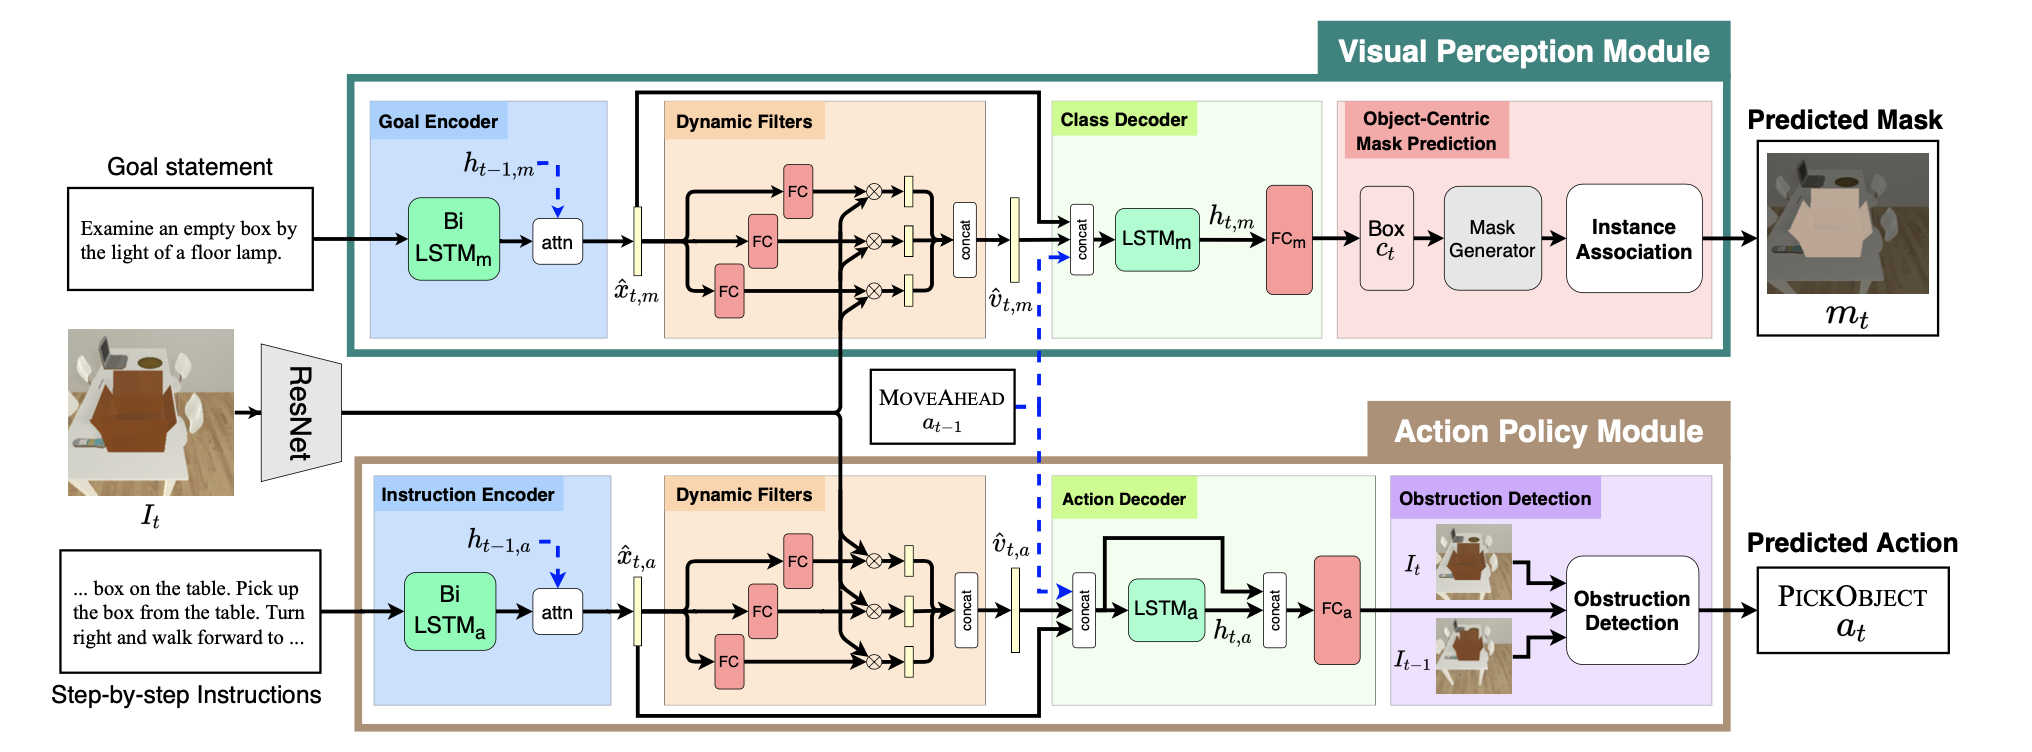
\includegraphics[width=\linewidth]{Reports/5-Proposed-Approach/system_arch.png}
%     \caption{Detailed model architecture from the MOCA paper.}
%     \label{fig:sys_arch}
% \end{figure*}

% \subsection{Improved Previous Step Mask Use}

% \subsection{Condition on Action to Predict Mask}

% In this subsection, we propose another strategy to reduce the amount of invalid actions caused by bad mask predictions. MOCA uses object-centric mask prediction whereby the first step is to predict the class of the object to interact with. Importantly, the current predicted action is not provided in target class prediction. This is a weakness because knowledge of what action to take would influence what object to act upon. Intuitively, one would be less likely to predict ``the fridge'' as the object if one knew the action was ``cut''. As a result, we will explore two methods of inputting the action to the mask prediction. For both methods, we would still use ``Instance Association in Time'' as defined in the MOCA paper. The first method is to concatenate the one-hot encoding of the action to the hidden state $h_{t,m}$ as below:

% \begin{equation}
% % \underset{x}{\operatorname{argmax}} 
%     c_t = \argmax_{k} FC_{m}([h_{t,m}; a_{t}]),
% \end{equation}

% where $c_t$ is the predicted class, $h_{t,m}$ is the hidden state of the VPM and $a_t$ is the predicted action of the current time step. The second method we will explore is to input the current action to the LSTM that outputs the hidden state $h_{t,m}$. In this case, equation 6 would change to the following: 

% \begin{equation}
%     h_{t,m} = LSTM_{m}([\hat{v}_{t,goal};\hat{x}_{t,goal};a_{t-1};\hat{x}_{t,instr};a_{t}])
% \end{equation}

% We will experiment on both methods and use the method with the better test performance.

% \subsection{Expected Difficulties and Proposed Mitigations}
% The primary difficulties that we expect to encounter involve the collection of action feasibility data. It will be trivial to collect data about navigation actions that don't require interactions with other objections. However, for interactive actions, we would like to gather data about whether any object in the image could be used with an interactive action. For example, for the action ``toggle'' we would like to know if there is any object in the image that can be ``toggled''. We plan to use the simulator to extract a mask for all objects in an image and query the simulator to verify if the actions are valid with any of the objects in the image.

% Another difficulty that we might encounter is that there might not be enough examples of infeasible actions along the training trajectories. One way in which we have already planned to mitigate this issue is by using focal loss \cite{lin2017focal}. This loss is similar to binary cross entropy but helps with class imbalance issues. In case this is not sufficient, we might have to sample additional trajectories that are semantically equivalent but that have more infeasible actions along their way (by infeasible actions we mean actions other than the golden actions at a given time step that are not feasible). This could be done by for example walking closer to objects that cannot be traversed but still reaching all stages of the training trajectory where the agent has to interact with an object.

\section{Experiments}

In this section, we will introduce the experiments based on our approaches. Note that due to time and resource constraints we did not evaluate the auxiliary loss approach which involved retraining the full MOCA model. The experiments only relate to the stand-along action feasibility module.

\subsection{Settings}
The model used for action feasibility prediction is a ResNet-18 with 2 fully connected layers. The threshold for positive prediction is 0.7 (value of logit), i.e. we only assign the sample as a feasible action if the output logits have a value greater than 0.7. To train such a model, we used Adam Optimizer with the learning rate $1\times10^{-5}$, batch size of 32, and trained model for 20 epochs. Weight decay is also used to prevent overfitting.

\subsection{Baselines}
We present below the two baselines that we plan to evaluate against our proposed approach along with the metrics that will be used for the evaluation.

\paragraph{Sequence-to-Sequence with Progress Monitor}
Along with collecting the ALFRED dataset, \citet{ALFRED20} proposed a baseline model for the task. They model the agent with a CNN-LSTM sequence-to-sequence architecture. A bidirectional-LSTM is used to generate a representation of the language instructions. A CNN encodes the visual input at each time step. And a decoder LSTM generates a sequence of low-level actions while attending over the encoded language and visual input. The model is trained to produce the actions and associated interaction masks from expert trajectories using imitation learning. The interaction mask is produced by a three layer deconvolution network trained with binary cross-entropy loss on ground-truth object segmentations.

The ALFRED task requires long action sequences to be completed. \citet{ALFRED20} propose to use two auxiliary losses to monitor the progress of the agent towards the completion of the task. The first loss involves predicting the current process (a scalar between 0 and 1) using the decoder hidden state, the visual input, the attended language instructions, and the previous action. In addition to the global progress, the model is trained to predict the number of sub-goals completed so far. 

\paragraph{Modular Object-Centric Approach (MOCA)}The Modular Object-Centric Approach (MOCA) \citep{singh2020moca} decomposes the interactive instruction following procedure into action, and policy generation tasks. Two modularized networks, named action policy module (APM) and visual perception module (VPM), deal with the action planning and visual localization tasks respectively via attentive filtering visual and language information. The method also proposed to use an obstruction detection module to address the difficulties in being stuck around the obstacles. The method successfully gains improvements from previous methods and is of state-of-the-art position.

For training MOCA, the objective function is composed of the loss for APM and VPM. To guide the discovery of objects, the basic objective functions are two cross-entropy losses that enforce the model to discover objects and the corresponding action classes for each step. Two loss functions helping to achieve subgoals, and monitor the overall progress.

\subsection{Metrics}
Here we discuss the metrics that we use to measure the performance in Alfred dataset. For the action feasibility model, we use classification accuracy and average precision as the metric to evaluate the model.

\paragraph{Task Success} To evaluate whether tasks have been successfully completed, the authors define two categories for success. For the task success metric, a score of 1 is given to a tasks trial when all of the goal conditions for that task have been met. If at least one goal condition is not met at the end of the sequence, a score of 0 is given. The main limitation of this metric is that the state-of-the-art models still perform poorly on the dataset, thus the percentage of tasks that meet every goal condition is very low.

\paragraph{Goal-Condition Success} To overcome this limitation, goal-condition success measures the proportion of goal-conditions that have been met for the task. For example, if the completion of a task requires 5 goal-conditions and only 2 are met during testing, a score of 0.4 will be given. In general, tasks with longer sequences of instructions have a lower goal-condition success as the directive is more complex. As a result, it is important to use the same test splits across experiments to keep the task length constant.

\paragraph{Path Weighted Metrics} A major limitation of both metrics is that one could attain a relatively high score by performing a long sequence of random acts. To overcome this, the authors perform path weighting (PW), which gives a lower score to action sequences that are long compared to the expert demonstration. The weighting follows the below equation where $p_s$ is the path weighted score, $s$ is the non-path weighted score, $L^*$ is the length of the expert demonstration sequence and $\hat{L}$ is the length of the predicted sequence.

$$p_s = s * \frac{L^{*}}{max(L^{*}, \hat{L} )}$$

\paragraph{Sub-Goal Evaluation} The last metric is sub-goal evaluation. Initially, the model is forced to follow the beginning part of the expert demonstration. Afterwards, the model must predict actions to complete the remaining sub-goals given the full textual instruction and the most recent image input. This metric allows analysis into how previous action sequences affect the prediction of future action sequences.

\subsection{Data Collection}

To train an action feasibility prediction model we need to gather a dataset with ground truth labels. Given time constraints, we focus on navigational actions and not interactive actions. Through experimentation, we found that the actions ``LookUp\_15``, ``LookDown\_15``, ``RotateLeft\_90`` and ``RotateRight\_90`` were always feasible. The only navigation action that could be infeasible was ``MoveAhead\_90``. Thus, our dataset consists of pairs of images and boolean values determining whether ``MoveAhead\_90`` was feasible or not for that image. An example of typical images can be observed in figure \autoref{fig:feas_infeas}.

\begin{figure}
    \centering
    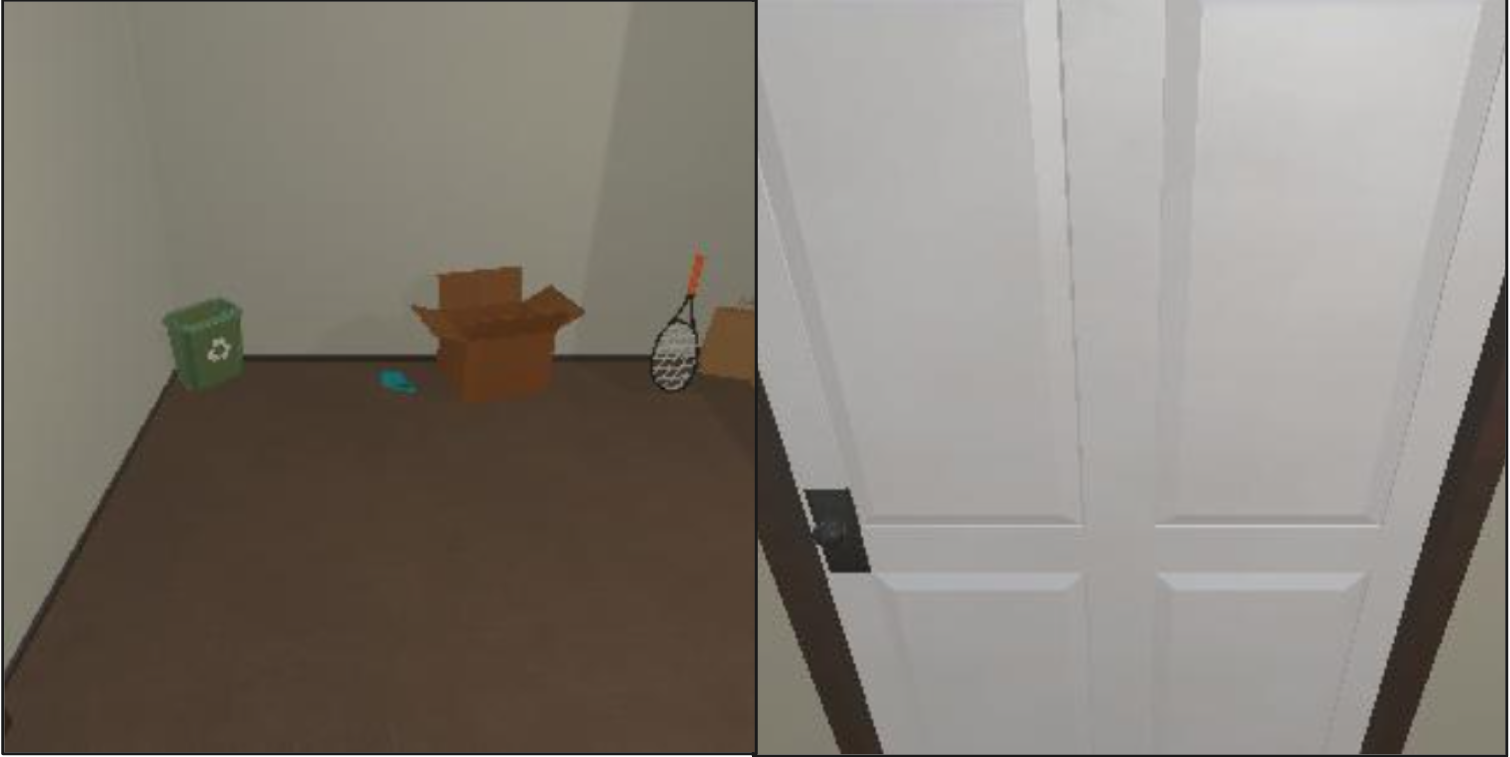
\includegraphics[width=\linewidth]{Reports/Report/feas_infeas.png}
    \caption{On the left is an image where ``MoveAhead\_15`` is feasible and on the right, ``MoveAhead\_15``is infeasible because there is a door blocking the path.}
    \label{fig:feas_infeas}
\end{figure}

In the training dataset, the same scene numbers are frequently reused with a variation in the layout of small items such as credit cards. Since the presence of these small items is largely irrelevant to whether or not moving ahead is feasible, we store one scene per scene number. For each unique scene, we get all the navigable, non-occupied x, y, z positions of which there is an average of 92 per scene. Within these positions, we rotate the agent four times and store an image as well as a boolean feasibility value for each rotation. We perform the same data collection on the unseen dataset in order to perform validation evaluations. There are 108 unique training scene numbers and 4 unique unseen scene numbers.

\subsection{Results}

\begin{table*}[]
    \centering
    \begin{tabular}{c|c|c|c|c}
    \toprule
    & \multicolumn{2}{c|}{Seen} & \multicolumn{2}{c}{Unseen} \\
    & Task (PW) & Goal-Cond (PW) & Task (PW) & Goal-Cond (PW) \\
    \midrule
    Seq2Seq + PM & 3.7 (2.1) & 10.0 (7.0) & 0.0 (0.0) & 6.9 (5.1) \\ 
    MOCA & \textbf{20.8} (14.4) & \textbf{29.7} (\textbf{22.6}) & 2.8 (1.4) & 12.8 (7.6) \\
    MOCA + Oracle All & 20.0 (\textbf{14.7}) & 29.5 (\textbf{22.6}) & 3.5 (2.0) & \textbf{14.2} (\textbf{8.8}) \\
    MOCA + Oracle Nav & 18.4 (12.9) & 27.5 (21.5) & \text{4.1} (\textbf{2.2}) & 14.1 (8.6) \\
    \bottomrule
    \end{tabular}
    \caption{Performance of MOCA+Oracle models.}
    \label{tab:results}
\end{table*}

In this section, we will introduce our results. We report results on two experiments to verify the effectiveness of our hypothesis. We would like to verify 1) if the action feasibility prediction could help, and 2) if it is possible to build such a model that predicts the feasibility actions. To answer the first question, we build an oracle feasibility predictor that perfectly predicts the feasibility of every navigational action, and we use the oracle outcome to prune the action space that the agent will operate on. When the oracle predict that the action is not feasible, we used two strategies to select the alternative action, includes 1) the most likely navigational action, and 2) the most likely action (including interactive actions). In the following, we will discuss these settings in detail. Here we report the results on Alfred validation set. 

\paragraph{Is action feasibility prediction going to help the task success?}

As mentioned above, to answer this question, we build two oracle models that perfectly predict the action feasibility and prune the action space. The performance of such a model is very important since it represents the upper bound performance of the actual action predictor, i.e., the performance of the trained action feasibility predictor should not be higher than that from the oracle. It also reveals some pitfalls and more fundamental issues in the robot. The results are shown in Table \ref{tab:results}. In the table, the MOCA term means the trained model from MOCA paper. Seq2Seq + PM is the model provided by alfred's original paper. MOCA + Oracle All means the alternative action selected is from all other actions except for the excluded ones. MOCA + Oracle Nav is the oracle model that selects only the navigational actions. 

It can be observed from the table that when the model has seen the room in the training set, the improvement from using the oracle predictor is very limited, while in the unseen cases there is a clear improvement. We believe this is due to the MOCA model already implicitly learning to predict the action feasibility during training in the seen environments. Furthermore, the MOCA has also a similar module inside it that helps avoid making mistakes by forcing the agent to turn after hitting the wall for some time, which thus makes the action feasibility prediction less useful. However, in the unseen cases, the MOCA is not very good at generalizing the from the training set and performs more infeasible actions on average. In these cases, the action feasibility prediction becomes helpful.

We also realize that there exist some more fundamental issues in the pipeline of MOCA. To be more specific, these models might have limitations in terms of planning, and using an action feasibility module might be too late to correct such fundamental issues. 

\paragraph{Is it possible to identify the feasibility of an action?}

\begin{figure}
    \centering
    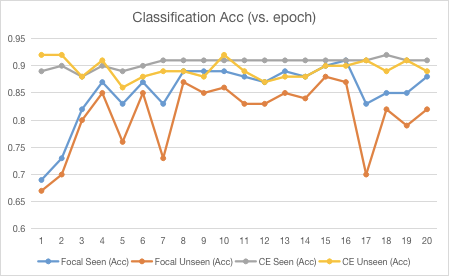
\includegraphics[width=\linewidth]{Fig0.png}
    \caption{Training plot}
    \label{fig:train_plot}
\end{figure}

To answer this question, we used the data collected with the approach described before and trained a separate model. In short, the answer to this question is yes, and the trained model transfers well from seen to unseen spaces, indicating the potential improvement in unseen cases, based on the results from the oracle model. From Table \ref{tab:trainedmodule}, we can observe that the module succeeds in predicting the action feasibility and reaches an overall accuracy in seen spaces of 90\%. While the performance in seen rooms is less informative, it's also observed that the prediction performance under unseen tasks is very competitive. We also compared the Focal Loss and Cross-Entropy Loss, showing that focal loss is helpful for the prediction of negative samples, it harms the performance in predicting positive samples. The plot showing the accuracy during training is shown in Figure \ref{fig:train_plot}.

\begin{table}[]
\centering
\resizebox{0.5\textwidth}{!}{%
\begin{tabular}{c|cccc}
         & Focal Seen & Focal Unseen & CE Seen & CE Unseen \\ \hline
Accuracy & 0.91       & 0.87         & 0.92    & 0.89      \\
Pos AP   & 0.85       & 0.81         & 0.97    & 0.95      \\
Neg AP   & 0.89       & 0.83         & 0.6     & 0.55     \\ \hline
\end{tabular}%
}
\caption{Action prediction performance from trained model, in the held-out validation dataset. Here Pos AP and neg AP is the average precision on positive and negative samples respectively. (Feasible action/ Infeasible action )}
\label{tab:trainedmodule}
\end{table}

\section{Conclusion}
In conclusion, in this project we explore the ALFRED task. We identified the issue of action feasibility as a possible area of improvement for the MOCA model. We proposed two approaches to solve this issue. Due to time constraints we only performed experiments on one of these approaches: the stand-along action feasibility module. This module, trained on data from the simulator, predicts the feasibility of the ``Move Ahead'' action given an image. Our model reaches 90\% accuracy in the seen cases with no significant loss in performance in unseen cases. Finally, our oracle experiments show that this external action feasibility module can improve performance in terms of success rate and goal conditioned success in the unseen scenes. 

In future work, we would like to explore the performance of the auxiliary loss approach which does not require a separate feasibility module but updates the MOCA model itself. Finally, our experiments indicate that other components of the MOCA model may be limiting the benefits from modeling action feasibility.


\clearpage
% Please use 
\bibliographystyle{acl_natbib}
\bibliography{references}

%\appendix



\end{document}
